\documentclass{beamer}
\usepackage[utf8]{inputenc}
\usepackage{url,hyperref,times}
\usepackage[T1]{fontenc}
\usepackage{verbatim,scalefnt,colortbl}
\usepackage[spanish]{babel}
\usepackage{graphics}
\usepackage{algorithm}
\usepackage{algorithmic}
\usepackage{program}
\mode<presentation>
{
%   \usetheme{CambridgeUS}
%   \usetheme{Berkeley}
  \usetheme{Madrid}

  \setbeamercovered{transparent}
  \setbeamertemplate{navigation symbols}{}
  \setbeamertemplate{footline}[page number]{}
  \usebackgroundtemplate{
\includegraphics[width=128mm, heigth=96mm]{dna-strand-code.jpg}}
  \setbeamercolor{normal text}{fg=black}
}
\usefonttheme{structureitalicserif}
\begin{document}
\title[]{Whole genome alignment in High Performance Computing environments}
\author[Julio García]{Julio César García Vizcaíno \and Directores: Antonio Espinosa, Juan Carlos Moure}
\institute[UAB]{
   
\includegraphics[scale=0.4]{caos.jpg}\\
   Computer Architecture \& Operating Systems Department\\
   Universitat Autónoma de Barcelona
}
\date[\today]{\today}
\pgfdeclareimage[height=0.3cm, width=0.6cm]{uab-logo.jpg}{uab-logo.jpg}
\logo{\pgfuseimage{uab-logo.jpg}}

\begin{frame}
  \titlepage
\end{frame}
\begin{frame}
  \frametitle{Contents}\tableofcontents
\end{frame}
\section{Problem definition}
\begin{frame}
\frametitle{Search of Maximal Exact Matches}
\begin{figure}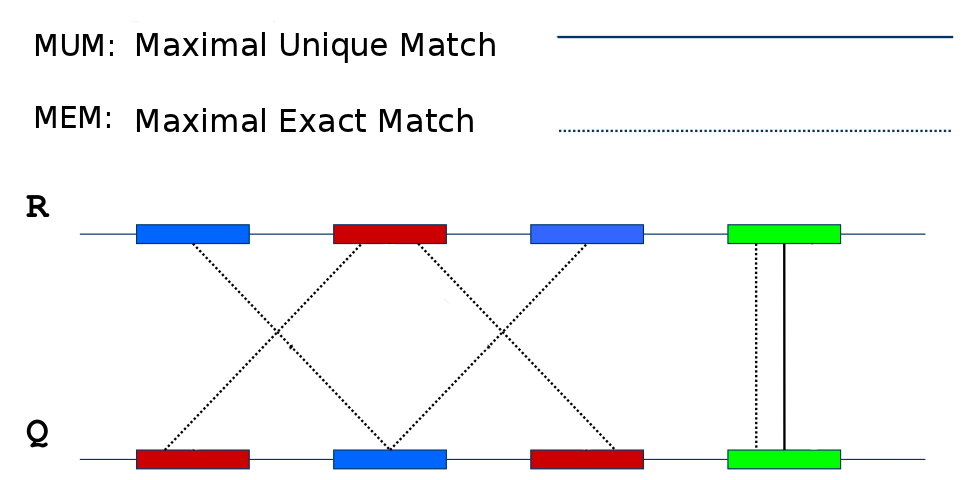
\includegraphics[scale=0.4]{mem.png}\end{figure}
\end{frame}
\begin{frame}
\frametitle{Genome alignment: search of Maximal Exact Matches}
\begin{figure}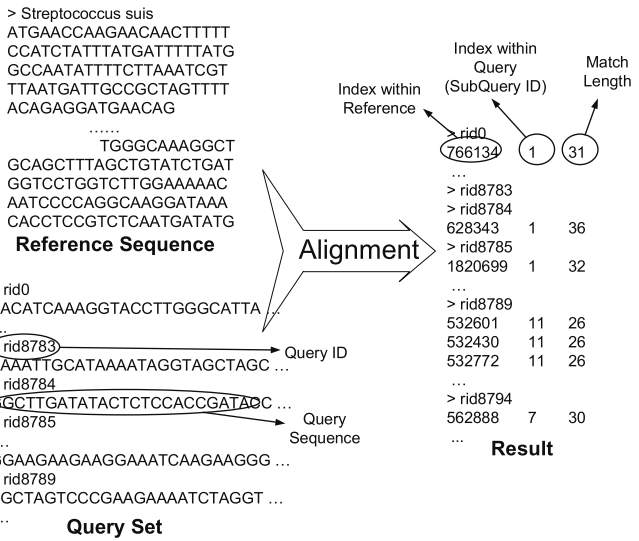
\includegraphics[scale=0.4]{problem.png}\end{figure}
\end{frame}
\begin{frame}
\frametitle{Search of Maximal Exact Matches}
\begin{figure}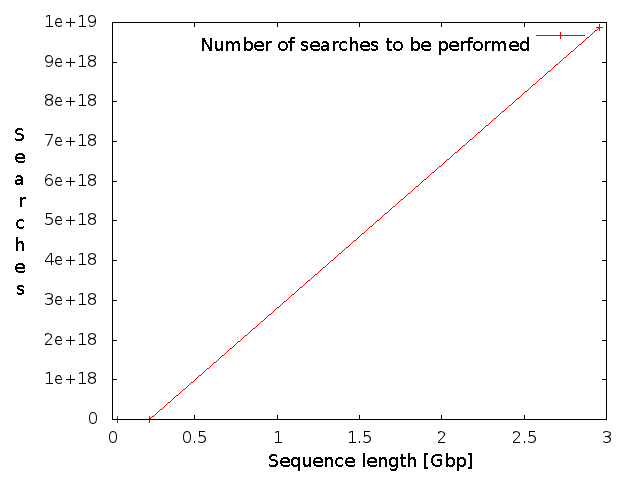
\includegraphics[scale=0.4]{search.png}\end{figure}
\end{frame}
\begin{frame}
 \frametitle{Ways of finding exact matches}
\begin{figure}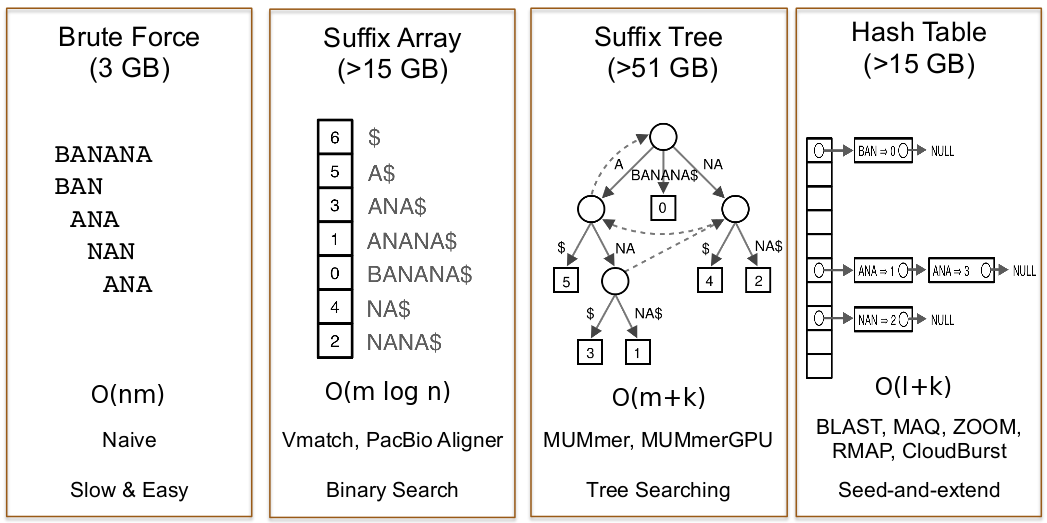
\includegraphics[scale=0.39]{state.png}\end{figure}
\end{frame}
%\begin{frame}
%  \frametitle{Brute force analysis}
%  \begin{block}{}
%    \begin{itemize}
%      \item Simple, easy to understand.
%      \item Reference length = n
%      \item Query length = m
%      \item Comparisons: $(n-m+l)*m$
%      \item Overall runtime: $O(nm)$
%    \end{itemize}
%  \end{block}
%\end{frame}
%\begin{frame}
%  \frametitle{Suffix arrays}
%  \begin{block}{}
%    \begin{itemize}
%      \item Sort every suffix of the genome.
%      \item Binary search.
%      \item Overall runtime: $O(m\log n)$
%    \end{itemize}
%  \end{block}
%\end{frame}
%\begin{frame}
%  \frametitle{Suffix trees}
%  \begin{block}{}
%    \begin{itemize}
%      \item It indexes \textbf{all} substrings of a sequence.
%      \item Nodes have at least 2 and at most 5 children (A,C,G,T,\$)
%      \item Query lookup in 2 phases:
%        \begin{itemize}
%          \item Walk along edges to find matches.
%          \item Walk subtree to find positions.
%        \end{itemize}
%      \item Number of Nodes/Edges: $O(n)$
%      \item Tree size: $O(n)$
%      \item Max Depth: $O(n)$
%      \item Construction time: $O(n)$
%        \begin{itemize}
%          \item Uses suffix links to jump between nodes without rechecking.
%          \item Tricky to implement, prove efficiency.
%        \end{itemize}
%    \end{itemize}
%  \end{block}
%\end{frame}
%\begin{frame}
%  \frametitle{Use of suffix tree}
%  \begin{block}{}
%    \begin{itemize}
%      \item Check for query: $O(m)$
%      \item Find all z occurences of a query: $O(m+z)$
%      \item Find maximal exact matches $O(m)$
%      \item Longest common substring $O(m)$
%    \end{itemize}
%  \end{block}
%\end{frame}
%\begin{frame}
%  \frametitle{Hash table}
%  \begin{block}{}
%    Running time:
%    \begin{itemize}
%      \item Construction: $0(n)$
%      \item Lookup: $O(l)+O(z)$
%    \end{itemize}
%    Seed and extend to find end-to-end exact matches.
%  \end{block}
%\end{frame}
\begin{frame}
  \frametitle{Traversal of suffix tree}
  \begin{figure}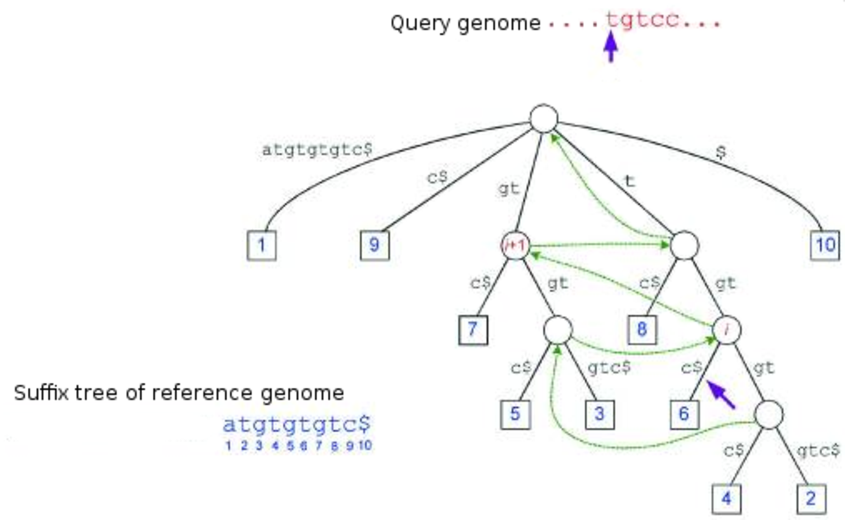
\includegraphics[scale=0.8]{st-mum.pdf}\end{figure}
\end{frame}
\section{Objectives}
\begin{frame}
 \frametitle{General objective}
 \begin{block}{General objective}
Speed up the search of exact matches (distributed) and adapt it to application MUMmer for its execution in HPC environments.
\end{block}
\end{frame}
\begin{frame}
\frametitle{Specific objective}
\begin{block}{}
\begin{itemize}
\item To have a data structure, efficient usage of memory and processor, that allows a quick search of maximal exact matches.
  \begin{itemize}
    \item Save relevant information for the search of matches.
    \item Be able to nimbly check the data structure.
  \end{itemize}
  \end{itemize}
\end{block}
\end{frame}
\begin{frame}
  \frametitle{Naive solution}
  \begin{figure}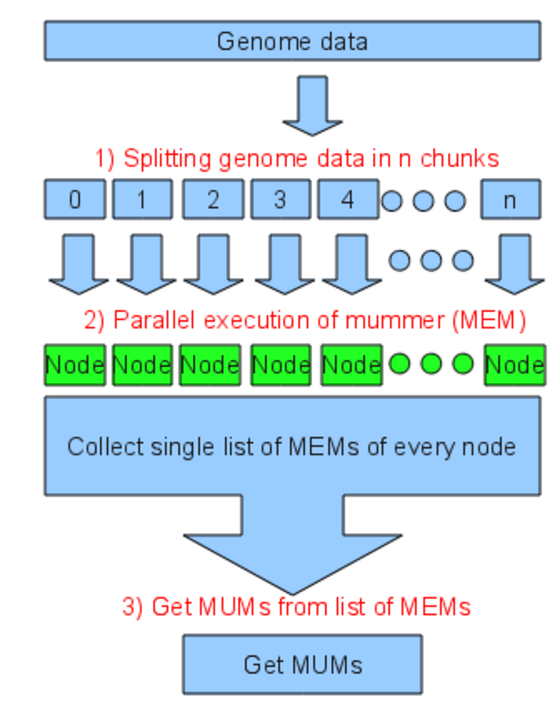
\includegraphics[scale=0.6]{algorithm.pdf}\end{figure}
\end{frame}
\begin{frame}
  \frametitle{Split sequence}
  \begin{columns}
    \begin{column}{0.5\textwidth}
  \begin{figure}
    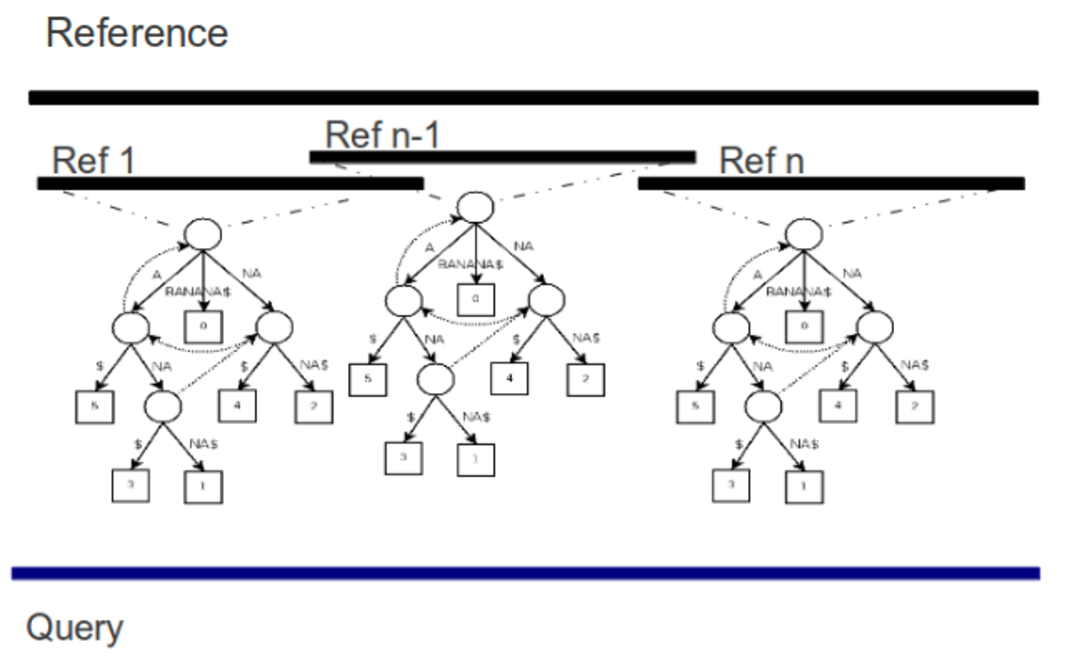
\includegraphics[scale=0.3]{split_ref.pdf}
  \end{figure}
  \end{column}
  \begin{column}{0.5\textwidth}
  \begin{figure}
    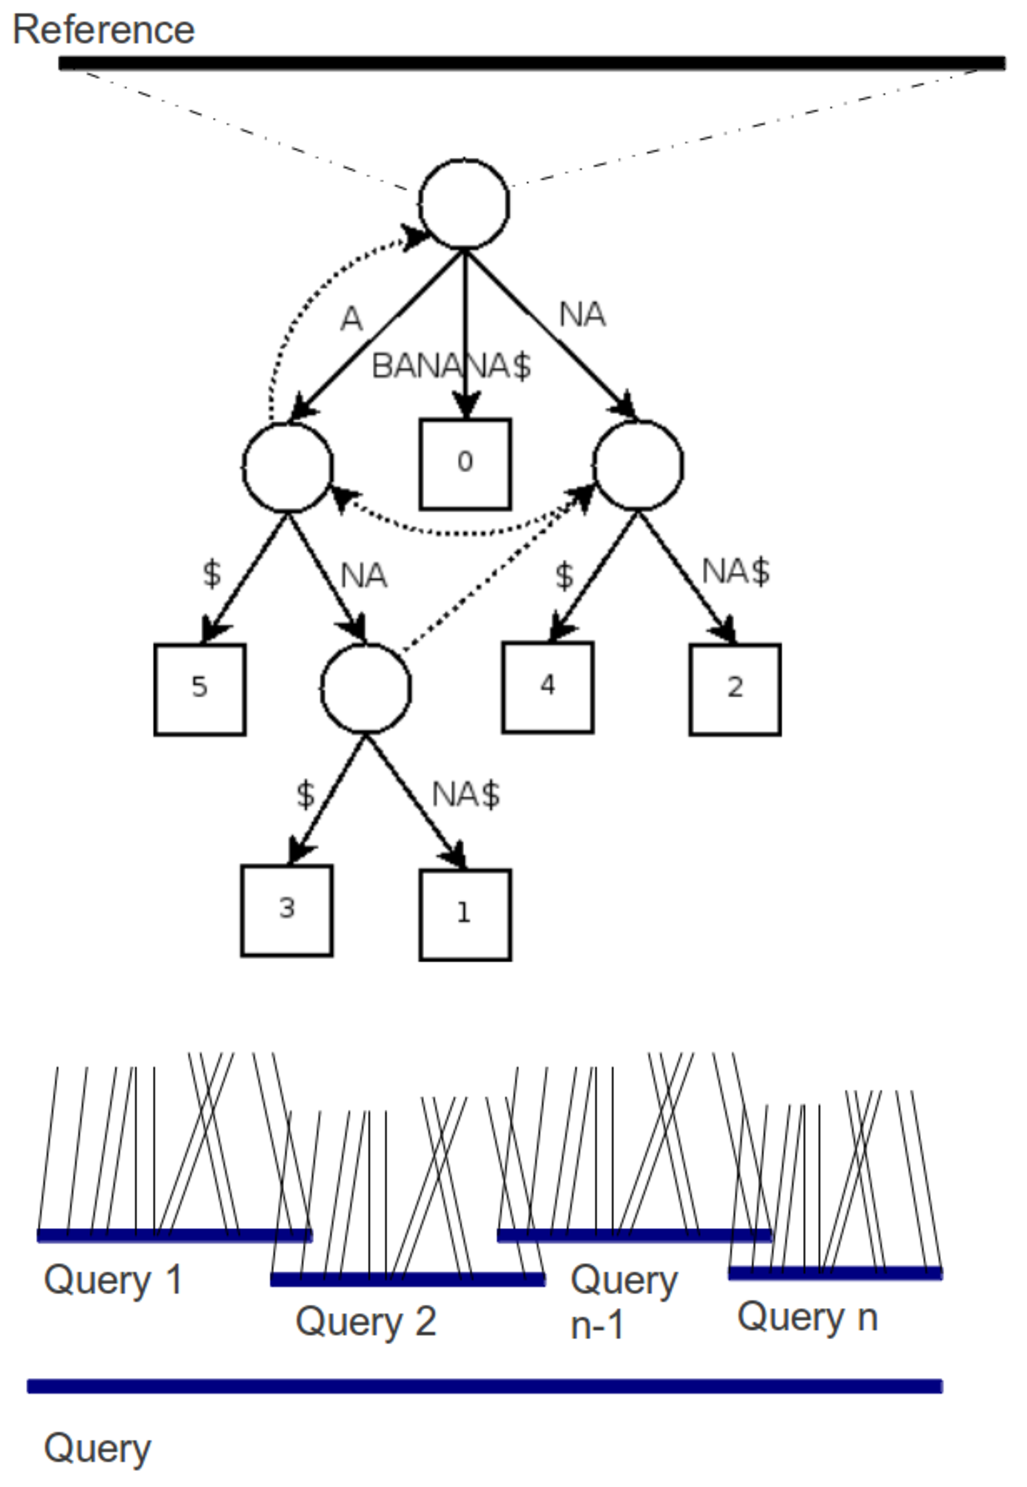
\includegraphics[scale=0.3]{split_qry.pdf}
  \end{figure}
\end{column}
\end{columns}
\end{frame}
\begin{frame}
\frametitle{Naive solution cont.}
  \begin{columns}
    \begin{column}{0.5\textwidth}
    \begin{figure}
      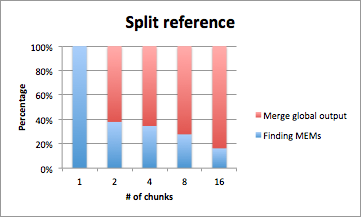
\includegraphics[scale=0.5]{ref_naive.png}
    \end{figure}
  \end{column}
  \begin{column}{0.5\textwidth}
  \begin{figure}
    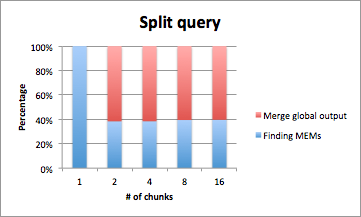
\includegraphics[scale=0.5]{qry_naive.png}
  \end{figure}
\end{column}
\end{columns}
\end{frame}
\section{Distributed suffix tree}
\begin{frame}
\frametitle{Distributed suffix tree}
\begin{block}{}
  \begin{itemize}
    \item New variant of the suffix tree.
    \item Handle of large strings efficiently.
    \item Based on linear time construction algorithm for subtrees of a suffix tree.
    \item It tackles the memory bottleneck problem by constructing these subtrees indepently and in parallel.
  \end{itemize}
\end{block}
\end{frame}
\begin{frame}
  \frametitle{Distributed suffix tree}
  \begin{figure}
    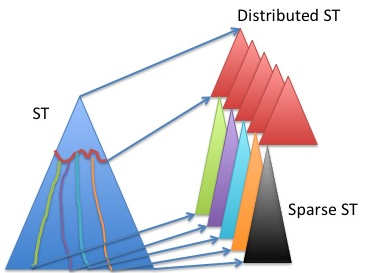
\includegraphics[scale=0.8]{distributed.png}
  \end{figure}
\end{frame}
\begin{frame}
  \frametitle{Traversal of a suffix tree}
  \begin{block}{}
   Every suffix of query (pointer) is searched in suffix tree. By using suffix links 
   we jump to other depth of suffix tree and we avoid to check $x$ characters.
 \end{block}
  \begin{figure}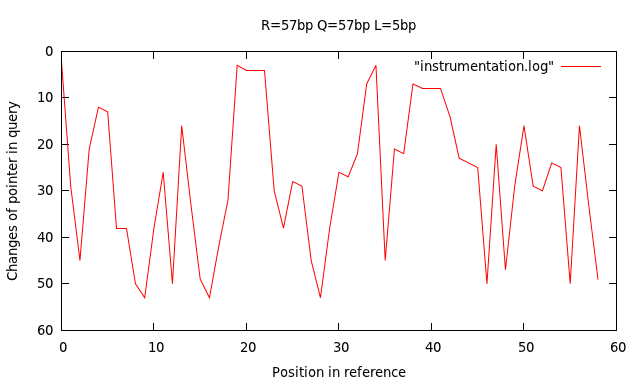
\includegraphics[scale=0.4]{r57-q57-l5.png}\end{figure}
\end{frame}
\begin{frame}
  \frametitle{Traversal of a suffix tree}
  \begin{block}{}
    The jumps in suffix tree are done while checking the parent node after finishing the last match.
  \end{block}
  \begin{figure}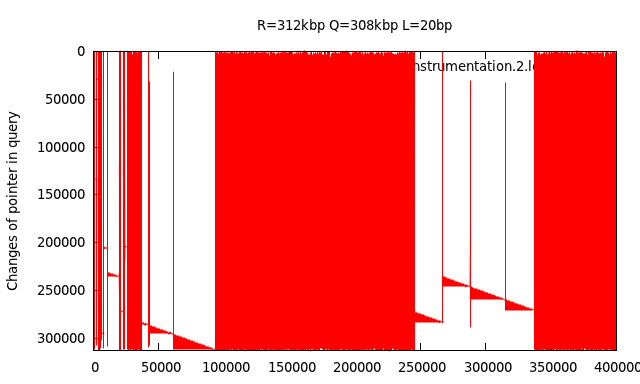
\includegraphics[scale=0.4]{r312kbp-q308kbp-l20.png}\end{figure}
\end{frame}
\begin{frame}
  \frametitle{Suffix links}
  \begin{block}{}
    The location of suffix links are made during suffix tree construction.
  \end{block}
  \begin{figure}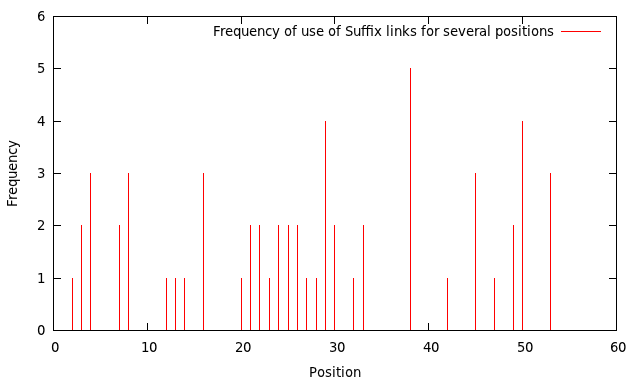
\includegraphics[scale=0.5]{histogram2.png}\end{figure}
\end{frame}
\begin{frame}
  \frametitle{Suffix links}
  \begin{block}{}
    The location of suffix links are more likely to be in deeper regions of suffix tree.
  \end{block}
  \begin{figure}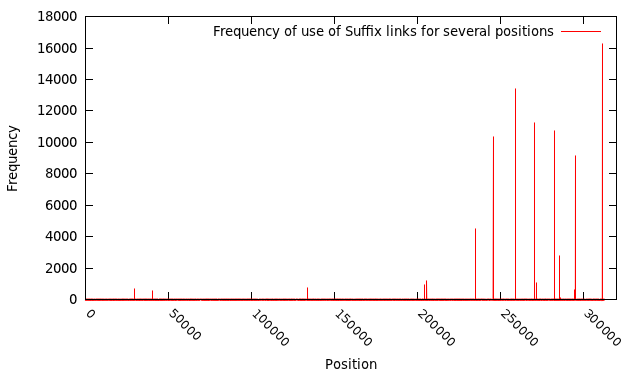
\includegraphics[scale=0.4]{histogram.png}\end{figure}
\end{frame}
\begin{frame}
  \frametitle{Access to suffix tree}
  \begin{block}{}
    Finding of maximal matches (path from root) are marked in suffix tree.\\
    Improved detection of maximal matches.
  \end{block}
  \begin{figure}
    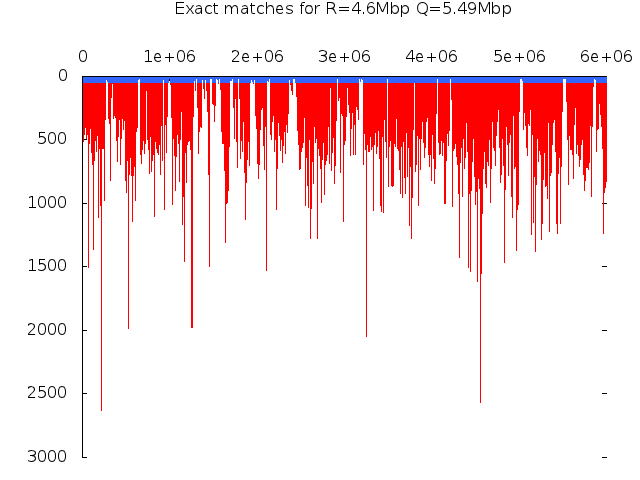
\includegraphics[scale=0.38]{freq.png}
  \end{figure}
\end{frame}
\begin{frame}
  \frametitle{Suffix tree: example}
  \begin{block}{}
  Standard suffix tree of aacacccacacaccacaaa\$ with standard suffix links.
\end{block}
  \begin{figure}
    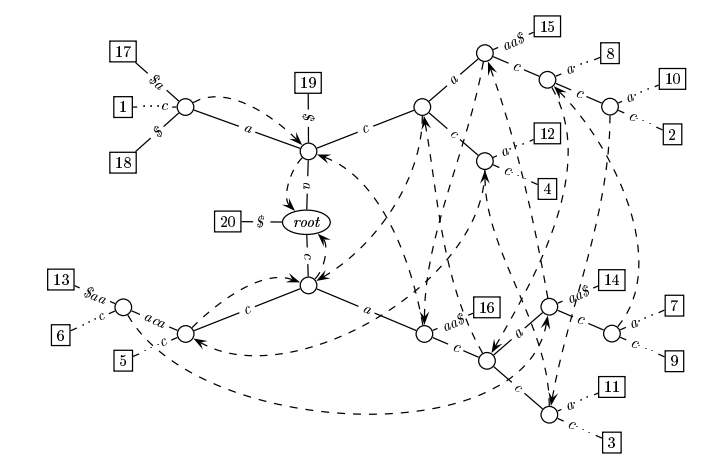
\includegraphics[scale=0.4]{dst1.png}
  \end{figure}
\end{frame}
\begin{frame}
  \frametitle{Distributed suffix tree}
  \begin{block}{}
  The SSTs for aacacccacacaccacaaa\$ with their respective root nodes labelled $r_{aa}, r_{ac}, r_{ca}, r_{cc}, r_{a\$}$ and $r_{\$}$.
\end{block}
\begin{figure} 
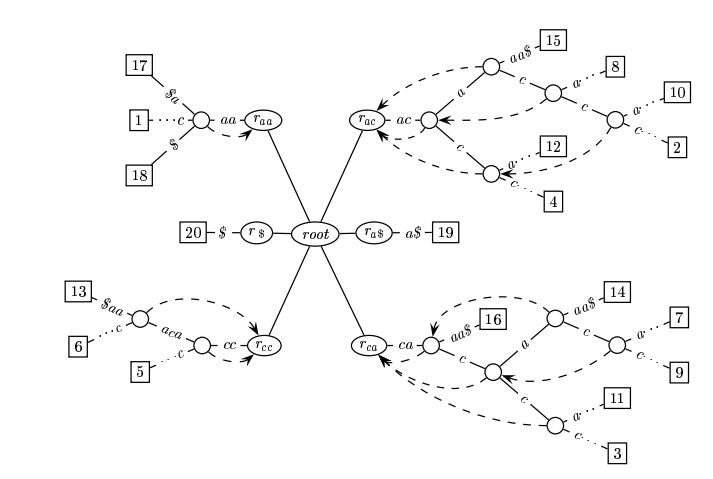
\includegraphics[scale=0.36]{dst2.png}
\end{figure}
\end{frame}
%\begin{frame}
%  \frametitle{Some definitions}
%  \begin{block}{Sparse suffix tree (SST)}
%    A sparse suffix tree (SST) of input string t to be a compacted trie of a subset of the suffixes of t.
%  \end{block}
%  \begin{block}{Distributed suffix tree (DST)}
%    A distributed suffix tree (DST) is simply a collection of SSTs defined in this way.
%  \end{block}
%  \begin{block}{Sparse suffix links}
%    Point to nodes that are within the same SST. 
%    \end{block}
%\end{frame}
%\begin{frame}
%  \frametitle{Some definition cont.}
%  \begin{block}{Valid set}
%    For a short prefix string $z$ and a set of start positions $V_{z}$.
%  \end{block}
%  \begin{block}{Valid suffix}
%    $s$ is a valid suffix for $I[i,j]$ if $s=t[k,j]$ for some $k \epsilon V_{z}$ and $k>i$ 
%  \end{block}
%  \begin{block}{Input pair}
%    $(t,V_{z})$ is an input pair if $V_{z}$ is the valid set (for t with respect to $z$).
%  \end{block}
%\end{frame}
%\begin{frame}
%  \frametitle{Sparse suffix link}
%  \begin{block}{}
%    Consider an input pair $(t,V_{z})$ and sparse suffix tree $T=sst(t,V_{z})$. Let $aw$ be nodal in $T$ and $v$ be the longest repeated suffix of $aw$ that occurs in $T$. A sparse suffix link is an unlabelled edge from $\overline{aw}$ to the root if $|v|<|z|$ and from $\overline{aw}$ to $\overline{v}$, otherwise.
%  \end{block}
%\end{frame}
%\begin{frame}
%  \frametitle{Further considerations}
%  \begin{block}{}
%    The suffix tree is an order of magnitude larger than the string being indexed.\\
%    For large input strings, the suffix tree cannot be acommodated in main memory.
%  \end{block}
%  \begin{block}{Solution}
%    Find a valid set of prefixes to partition the suffix tree into sparse suffix trees that can be built in main memory.
%  \end{block}
%\end{frame}
%\begin{frame}
%  \frametitle{Balanced distributed suffix tree}
%  \begin{block}{}
%    Let $f(p)$ denote the number of times prefix poccurs in S. Let MSSTS (Maximum Sparse Suffix Tree Size) denote the maximum amount of memory space in bytes that can be allotted to the sparse suffix tree during tree construction. Let NS denote the size of a suffix tree node in bytes.
%  \end{block}
%  \begin{block}{Goal}
%    Find a set of valid input pair such that $\forall p \epsilon V_{z}, 2xf(p)<\frac{MSSTS}{NS}$.
%  \end{block}
%\end{frame}
\section{Distributed and parallel search of maximal matches}
%\begin{frame}
%  \frametitle{Distributed and parallel search of maximal matches}
%  \begin{block}{Split query sequence}
%    Consider a query sequence of length $n$ and a distributed suffix tree. How to find the maximal matches of query sequence: acaccacaaccaacaaaaccaccacacc in distributed suffix tree?
% \end{block}
%\end{frame}
\begin{frame}
  \frametitle{Distributed and parallel search of maximal matches}
  \begin{figure}
    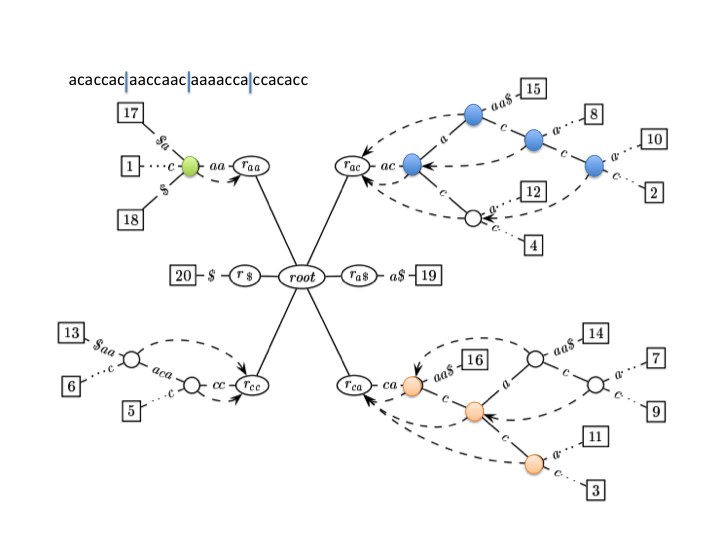
\includegraphics[scale=0.4]{dst_search.png}
  \end{figure}
\end{frame}
\section{Conclusions}
    \begin{frame}
    \frametitle{Conclusions}
    \begin{block}{First year}
It has been adapted a data structure which can be deployed in HPC environments.\\
It may be used to implement parallel and distributed techniques for search of maximal matches.\\
This data structure is able of handling large input sequences to search maximal exact matches.
\end{block}
\end{frame}
\begin{frame}
  \frametitle{Future work}
\begin{block}{}
Perform massive searchs of maximal matches: design and test a parallel and distributed algorithm to perform the search of maximal matches in HPC environments.
\end{block}
\end{frame}
\section{}
\begin{frame}
  \begin{center}
    \Huge{Thanks!}
\end{center}
\end{frame}
\begin{frame}
  \titlepage
\end{frame}
\end{document}
